\documentclass{ximera}
\input{../preamble.tex}
\author{}
\license{Creative Commons 4.0 By-NC-SA}
%\outcome{Compute an antiderivative using basic formulas}
\begin{document}
\begin{exercise}
Find the area of the polygon shown below.
  \begin{center}
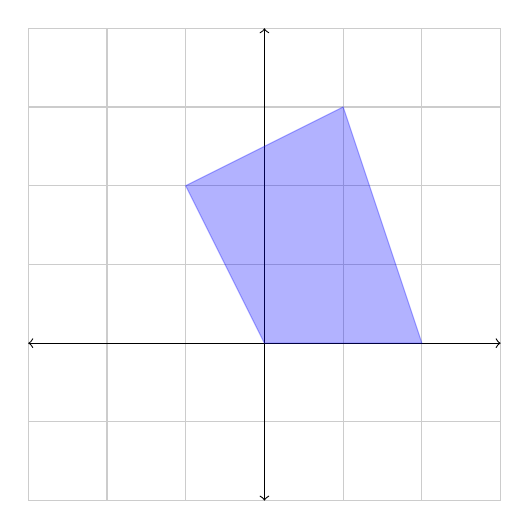
\begin{tikzpicture}[scale=1]
\draw[thin,gray!40] (-3,-2) grid (3,4);
  \draw[<->] (-3,0)--(3,0);
  \draw[<->] (0,-2)--(0,4);
  \filldraw[blue, opacity=0.3](0,0)--(-1,2)--(1,3)--(2,0)--cycle;
 \end{tikzpicture}
\end{center}  

\begin{hint}
    See Example \ref{exp:polyArea} and Formula \ref{form:areaofparallelogramdeterminant}.
\end{hint}

$$\text{Area}=\answer{5.5}\,\text{square units}$$
 \end{exercise}
 
\end{document}